\documentclass[12pt]{article}
\usepackage[margin=1in]{geometry} 
\usepackage{graphicx}
\usepackage{amsmath,amsthm,amssymb}
\usepackage{hyperref}

\title{
    \textbf{Assignment 1} \\ 
    \textbf{AI2000} \\
    \textbf{Foundations of Machine Learning}
}

\author{
    \textbf{Darpan Gaur} \\
    \textbf{CO21BTECH11004}
}


\date{}

\begin{document}
\maketitle

\hrulefill

\section*{Problem 1: k-NN}
\subsection*{Part a}
\begin{itemize}
    \item k = n, majority vote will be taken for all data points. As both classes have equal number of data points, 
          same class will be assigned to all data points. So, training error will be high (underfitting).
    \item n $>$ k $>$ 1, As k decrease from n to 1, training error will decreases as neighbood is shirnking. Transition from underfitting to overfitting.
    \item k = 1, each data point will be assigned the class of its nearest neighbour. So, training error will be zero (overfitting).
\end{itemize}
\subsection*{Part b}
% add a link to the figure
Refer to the figure \hyperref[fig: Figure 1]{1} below for the plot of training error vs k.
\begin{itemize}
    \item k=n, majority vote will be taken for all data points. As both classes have equal number of data points, 
          same class will be assigned to all data points. So, generalization error will be high (underfitting).
    \item n $>$ k $>$ 1, As k decreases, the generalization error decreases as neighbood is shirnking, model is becmoing better.
            But starts increasing after a certain point, as model is starts overfitting the training data.
    \item k=1, Train error will be 0, but on unseen data error will be high as model doesn't generalize well on unseen data.
\end{itemize}

% Add figure
\begin{figure}[h]
    \centering
    \label{fig: Figure 1}
    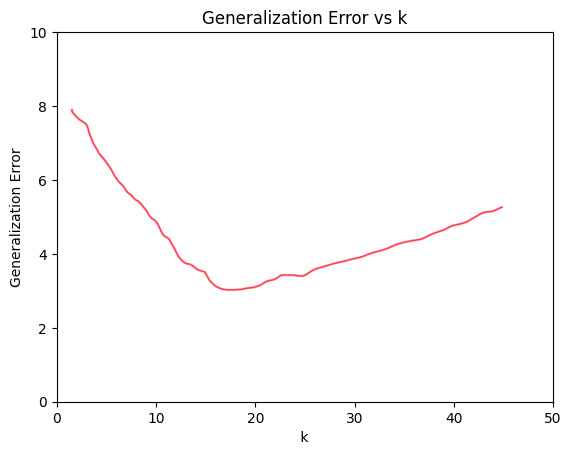
\includegraphics[width=0.5\textwidth]{../generalizationError.png}
    \caption{Generalization error vs k}
\end{figure}

\subsection*{Part c}
\begin{itemize}
    \item 1-NN classifier maked decision based on the nearest neighbour using euclidean distance.
            Hence, decision boundary will be non-linear and sensitive discontinuities in the data.
    \item Univatriate decision tree makes decision based on the threshold of a single feature.
            Hence, splits will be straight lines parallel to the axis, decision boundary will be linear.
    \item For example, consider two classes of data points in 2D space, seperate by diagonal line by 1-NN. 
            While univate decision tree will require mulitple horizointal and vertical lines to approximate the diagonal line, 
            and will not be able to capture the diagonal line.
    \item Moreover, as we increase dimensions of data or overlapping of data, univariate decision tree will not be able
            to capture the complex decision boundary, while 1-NN will be able to capture the complex decision boundary.
\end{itemize}

\section*{Problem 2: Bayes Classifier}
\subsection*{Part a}

For class $i$ maximum likelihood estimates for $\mu_i$, $\sigma^2_i$ and $p_i$ are given by,  
\begin{equation}
    \hat{\mu}_i = \frac{1}{N_i} \sum_{n=1}^{N_i} x_n
\end{equation}

\begin{equation}
    \hat{\sigma}^2_i = \frac{1}{N_i} \sum_{n=1}^{N_i} (x_n - \hat{\mu}_i)^2
\end{equation}

\begin{equation}
    {p}_i = \frac{N_i}{\sum_{j=1}^{K} N_j}
\end{equation}

For class 1, 
\begin{equation}
    \hat{\mu}_1 = \frac{1}{10} \times (0.5 + 0.1 + 0.2 + 0.4 + 0.3 + 0.2 + 0.2 + 0.1 + 0.35 + 0.25) = 0.26
    \nonumber
\end{equation}

Given, $\hat {\sigma}^2_1 = 0.0149$

\begin{equation}
    \text{Class propbability: } 
    p_1 = \frac{10}{10 + 4} = 0.7143
    \nonumber
\end{equation}

For class 2,
\begin{equation}
    \hat{\mu}_2 = \frac{1}{4} \times (0.9 + 0.8 + 0.75 + 1.0) = 0.8625
    \nonumber
\end{equation}

Given, $\hat {\sigma}^2_2 = 0.0092$

\begin{equation}
    \text{Class propbability: } 
    p_2 = \frac{4}{10 + 4} = 0.2857
    \nonumber
\end{equation}

The propbability that data point $x$ belongs to class $y$ is given by,
\begin{equation}
    p(y|x) = \frac{p(x|y)p(y)}{p(x)} 
    = \frac{p(x|y)p(y)}{\sum_{j=1}^{K} p(x|y=j)p(j)}
\end{equation}

As guassian distribution is given,
\begin{equation}
    p(x|y) = \frac{1}{\sqrt{2\pi\sigma^2}} \exp\left(-\frac{(x-\mu)^2}{2\sigma^2}\right)
\end{equation}

Propbability that data point $x = 0.6$ belongs to class 1 is given by,
\begin{equation}
    p(1|x=0.6) = \frac{p(x=0.6|1)p(1)}{p(x=0.6|1)p(1) + p(x=0.6|2)p(2)}
\end{equation}

\begin{equation}
    p(x=0.6|1) = \frac{1}{\sqrt{2\pi\hat{\sigma}^2_1}} \exp\left(-\frac{(0.6-\hat{\mu}_1)^2}{2\hat{\sigma}^2_1}\right)
    = \frac{1}{\sqrt{2\pi0.0149}} \exp\left(-\frac{(0.6-0.26)^2}{2\times0.0149}\right)
    = 0.0675
    \nonumber
\end{equation}

\begin{equation}
    p(x=0.6|2) = \frac{1}{\sqrt{2\pi\hat{\sigma}^2_2}} \exp\left(-\frac{(0.6-\hat{\mu}_2)^2}{2\hat{\sigma}^2_2}\right)
    = \frac{1}{\sqrt{2\pi0.0092}} \exp\left(-\frac{(0.6-0.8625)^2}{2\times0.0092}\right)
    = 0.0983
    \nonumber
\end{equation}

\begin{equation}
    p(1|x=0.6) = \frac{0.0675 \times 0.7143}{0.0675 \times 0.7143 + 0.0983 \times 0.2857}
    \approx 0.631
    \nonumber
\end{equation}

\subsection*{Part b}
p(politics) = 0.5, p(sports) = 0.5, as both have equal data points.\\
For $x_{politics}$, \\
p(goal=x(goal)$|$politics) = $\frac{\text{Number of times goal=x(goal) = 1 in politics}}{\text{Total politics data points}} = \frac{2}{6} $ \\
Similarly, \\ 
P(football=x(football)$|$politics) = $\frac{5}{6}$ , P(golf=x(golf)$|$politics) = $\frac{5}{6}$, P(defense=x(defense)$|$politics) = $\frac{5}{6}$, P(offence=x(offense)$|$politics) = $\frac{5}{6}$ \\
P(wicket=x(wicket)$|$politics) = $\frac{1}{6}$, P(office=x(office)$|$politics) = $\frac{4}{6}$, P(strategy=x(strategy)$|$politics) = $\frac{1}{6}$ \\
\\
In vector form, \\
P(x$|$politics) = $\begin{bmatrix} \frac{2}{6}  \frac{5}{6}  \frac{5}{6}  \frac{5}{6} \frac{5}{6}  \frac{1}{6}  \frac{4}{6}  \frac{1}{6} \end{bmatrix}$
\\
\\
P(x$|$sport) = $\begin{bmatrix} \frac{4}{6}  \frac{2}{6}  \frac{5}{6}  \frac{4}{6}  \frac{1}{6} \frac{1}{6}  \frac{0}{6}  \frac{5}{6} \end{bmatrix}$

\begin{equation*}
    p(y|x) = \frac{p(x|y)p(y)}{p(x)} = \frac{p(x|y)p(y)}{\sum_{j=1}^{K} p(x|y=j)p(j)}
\end{equation*}

\begin{equation*}
    p(politics|x) = \frac{p(x|politics)p(politics)}{p(x|politics)p(politics) + p(x|sports)p(sports)} = \frac{0.00148843545}{0.00148843545 + 0} = 1
\end{equation*}

\section*{Problem 3: Decision Trees}
\subsection*{Part a}
Implemented univariate decision tree using entropy and information gain.\\
Refer the .ipynb file. \\
Accuracy with train-test split of 75-25 is 85\%. 

\subsection*{Part b}
With 10-fold cross validation, accuracy is 87.2955\% (approx). \\
There is an increase of 2.3\% in accuracy with 10-fold cross validation as compared to train-test split. \\ 

\subsection*{Part c}
Gini index instead of entropy \\
Accuracy with train-test split of 75-25 is 85.25\%, an increase of 0.25\%. \\
Accuracy with 10-fold cross validation is 87.61\%, an increase of 0.32\%. \\
There is slight implrovement by using gini index instead of entropy as both metrics are similar. The computation time was slightly 
less for gini index as compared to entropy as gini index is computationally less expensive than entropy. \\
\\
Prune the tree after splitting for better generalization. \\
Change min\_samples and max\_depth, for pruning and to avoid overfitting. \\
Accuracy with 10-fold cross validation is 87.54\%, an increase of 0.25\% \\
Pruning the tree after splitting, helps in reducing overfitting and improves generalization. \\
Here as we are contraining the depth of the tree, here we can be a significant reduciotn in computation time. \\

\section*{Problem 4: Method Comparison}
\subsection*{Part a}
Let dataset size (number of training examples) be $n$ and number of features be $d$. \\
\textbf{K-Nearest Neighbours:} 
\begin{itemize}
    \item \textbf{Training  :} $O(1)$. KNN is a lazy learning algorithm, it dosen't learn a model from the training data.
    \item \textbf{Inference :} $O(nd)$. For each query, we need to calculate the distance of the query point from all the training points.
                                Each distance calculation takes $O(d)$ time as there are $d$ features. So, total time complexity is $O(nd)$.
\end{itemize}  
\textbf{Decision Trees:}
\begin{itemize}
    \item \textbf{Training  :} $O(nd\log n)$. At each node, algo searches for the best feature and threshold to split, 
                                evaluating all $d$ features across all $n$ training examples.
                                This process is repeated for each node, and there are $O(\log n)$ nodes in a balanced tree.
    \item \textbf{Inference :} $O(dlog n)$. For each query, we need to traverse the tree from root to a leaf node.
                                This process is repeated for each query, and there are $O(\log n)$ nodes in a balanced tree.
\end{itemize}
\textbf{Naive Bayes:}
\begin{itemize}
    \item \textbf{Training  :} $O(nd)$. Calulating prior propbability takes $O(n)$ time and calculating likelihood takes $O(nd)$ time for binary features.
                                Overall time complexity is $O(nd)$.
    \item \textbf{Inference :} $O(d)$. For each query, classifier computes propbability by multiplying/summation of the likelihood of each feature,
                                using precomputed likelihoods, the time complexity is $O(d)$.
\end{itemize}

\subsection*{Part b}
If cases not mentioned, assume for all four $n$ and $d$ cases.
\textbf{K-Nearest Neighbours:}
\begin{itemize}
    \item Weaknesses: 
           \begin{itemize}
                \item For large $n$ - large $d$, large $n$ - small $d$, small $n$ - large $d$, $nd$ is large, 
                        so slow infernece, high memory usage as it stores all training data.
                \item For small $n$ - small $d$, $nd$ is small, so fast inference, low memory usage.
                \item For large $d$, curse of dimensionality, as distance between points becomes meaningless.
            \end{itemize}
    \item Strengths:
            \begin{itemize}
                \item For small $n$ - small $d$, Simple to implement, no training time, easy to understand.
                \item Non-parametric, can capture complex decision boundaries.
            \end{itemize}
\end{itemize}

\textbf{Decision Trees:}
\begin{itemize}
    \item Strengths: 
            \begin{itemize}
                \item For large $n$ - large $d$, infernece is fast, as tree traversal is $O(\log n)$. Good feature selections, handles high dimensional data.
                \item For large $n$ - small $d$, faster inference.
                \item For small $n$ - large $d$, pruning can be used to avoid overfitting, due to high dimensional data.
                \item For small $d$, simple to understand, easy to interpret.
            \end{itemize}
    \item Weaknesses:
            \begin{itemize}
                \item For large $n$ - large $d$, $nd\log n$ is large, so slow training, prone to overfitting as time becomes very deep and complex.
                \item For large $n$ - small $d$, slow training.
                \item For small $n$ - large $d$, prone to overfitting, as limited data points, difficulty to find generalizable patterns.
                \item For small $n$ - small $d$, overfitting may occur.
            \end{itemize}
\end{itemize}

\textbf{Naive Bayes:}
\begin{itemize}
   \item Strengths:
            \begin{itemize}
                \item For large $n$ - large $d$, fast infernece.
                \item For large $n$ - small $d$, fast inference, Independent assumption good with less features.
                \item For small $n$ - large $d$, Efficient with limited data, avoids overfitting.
                \item For small $n$ - small $d$, Well suited, due to its simplicity and ability to generalize well on small data.
            \end{itemize}
    \item Weaknesses:
            \begin{itemize}
                \item For large $n$ - large $d$, Independent assumption may be unrealistic, leading to drop in performance.
                \item For large $n$ - small $d$, Training time would be increased. Correlation between features may affect the performance.
                \item For small $n$ - large $d$, Independent assumption as large number of features.
                \item For small $n$ - small $d$, Overfitting may occur.
            \end{itemize}
\end{itemize}

\end{document}
